\section{The Early Visual System}
\label{sec:EarlyVisualSystem}
\begin{prin}[Retinal Signal Conversion]
  \label{prin:retina}
  The conversion of a light stimulus into an electrical signal and ultimately an action potential sequence occurs in the retina.
  The retina is roughly composed of 3 layers of cells, \emph{photoreceptor cells}, \emph{bipolar cells} and \emph{ganglion cells}. First, photoreceptor cells convert light signals into electrical signals. And then, bipolar cells are responsible for sorting and processing these electrical signals. Finally, ganglion cells will convert electrical signals into action potential sequences.
   In the intact eye, counterintuitively, light enters through the side opposite from the photoreceptors because Vertebrate retinal cell layers are arranged in reverse order of signaling.
\end{prin}

\begin{rem}
   Changing membrane potentials is adequate for signaling within the retina, where distances are small. However, it is inadequate for the task of conveying information from the retina to the brain. Thus, the ganglion cells are needed.
\end{rem}

\begin{exm}
  The following figure A is an anatomical diagram showing the five principal cell types of the retina and figure B is a rough circuit diagram and intracellular recordings made in neurons of the retina of a mud puppy (an amphibian). The rod cells, especially the one on the left side of figure B, are hyperpolarized by the light flash. This electrical signal is passed along to bipolar and horizontal cells through synaptic connections. Note that in one of the bipolar cells, the signal has been inverted, leading to depolarization. Pluses and minuses represent excitatory and inhibitory synapses, respectively.
  The two retinal ganglion cells shown in the figure have different responses and transmit different sequences of action potentials. $G_2$ fires while the light is on, and $G_1$ fires when it turns off. These are called \emph{ON} and \emph{OFF responses}, respectively
  \begin{center}
    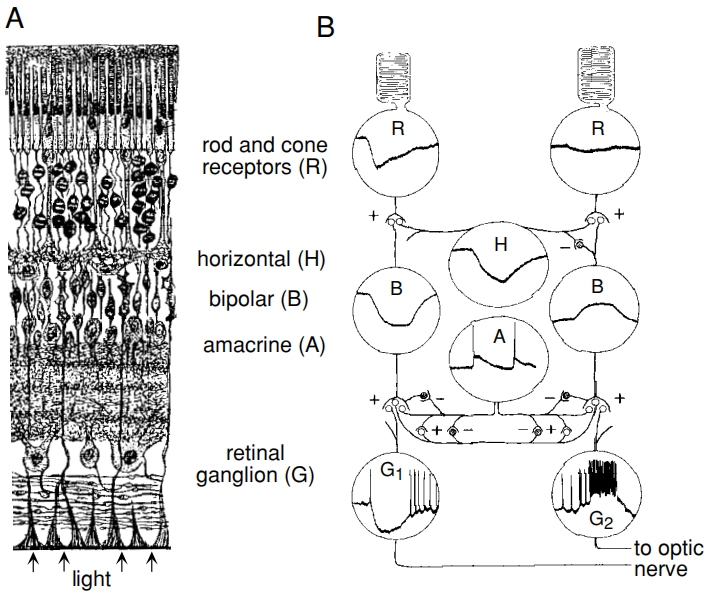
\includegraphics[scale=0.25]{./png/dogRetina}
  \end{center}
\end{exm}

\begin{defn}
  \label{defn:opticNerve}
  The output neurons of the retina are the retinal ganglion cells, whose axons form the \emph{optic nerve}.
\end{defn}

\begin{prin}[Visual Pathway]
  \label{prin:visualPathway}
  As the following figure shows, the optic nerve carry information from each visual hemifield up to the \emph{optic chiasm}, where some retinal ganglion cell axons cross the midline at the optic chiasm, and then to the LGN. Cells in this nucleus send their axons along the optic radiation to the primary visual cortex.
  \begin{center}
    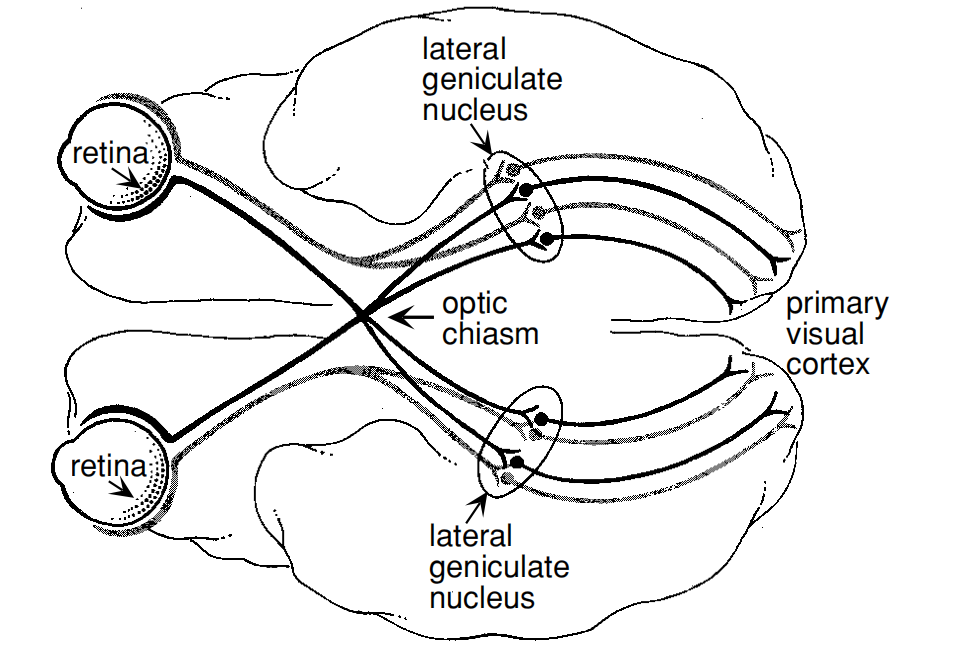
\includegraphics[scale=0.2]{./png/visualPathway}
  \end{center}
\end{prin}

\begin{defn}
  \label{def:visualReceptiveField}
  The restricted regions of the visual field where light stimuli could active Neurons in the retina, LGN, and primary visual cortex is called \emph{receptive fields of} the corresponding \emph{visual neuron}.
\end{defn}

\begin{asm}
  \label{asm:OutsideRecept}
  Patterns of illumination outside the receptive field of a given neuron cannot generate a response directly, although they can significantly affect responses to stimuli within the receptive field. We do not consider such effects, although they are of considerable experimental and theoretical interest.
\end{asm}

\begin{rem}
  Within the receptive fields, there are regions where illumination higher than the background light intensity enhances firing, and other regions where lower illumination enhances firing. The spatial arrangement of these regions determines the selectivity of the neuron to different inputs. The term \emph{receptive field} is often generalized to refer not only to the overall region where light affects neuronal firing, but also to the spatial and temporal structure within this region.
\end{rem}

\begin{defn}
  \label{simpleComplexCells}
  Visually responsive neurons in the retina, LGN, and primary visual cortex are divided into two classes, depending on whether or not the contributions from different locations within the visual field sum linearly. \emph{Simple cells} in primary visual cortex appear to satisfy this assumption. \emph{Complex cells} in primary visual cortex do not show linear summation across the spatial receptive field, and nonlinearities must be included in descriptions of their responses.
\end{defn}

\begin{asm}
  \label{asm:light}
  To streamline the discussion in this chapter, we consider only gray-scale images, although the methods presented can be extended to include color. We also restrict the discussion to two-dimensional visual images, ignoring how visual responses depend on viewing distance and encode depth.
\end{asm}

\begin{rem}
  In discussing the response properties of retinal, LGN, and V1 neurons, we do not follow the path of the visual signal, nor the historical order of experimentation, but instead begin with primary visual cortex and then move back to the LGN and retina. And the emphasis of this chapter is on properties of individual neurons.
\end{rem}

\subsection{The Retinotopic Map}
\label{sec:retinotopicMap}
\begin{defn}
  \label{def:retinotopicMap}
  The \emph{retinotopic map} is a map from the visual world to the cortical surface that make sure neighboring points in a visual image evoke activity in neighboring regions of visual cortex. 
\end{defn}

\begin{rem}
  A striking feature of most visual areas in the brain, including primary visual cortex, is that the visual world is mapped onto the cortical surface in this topographic manner.
  The retinotopic map refers to the transformation from the coordinates of the visual world to the corresponding locations on the cortical surface.
\end{rem}

\begin{defn}
  \label{def:fixationPoint}
  The image point that focuses onto the fovea or center of the retina is called the \emph{fixation point}.
\end{defn}

\begin{defn}
  \label{def:sphericalCoord}
  Locations on a sphere can be represented using the same longitude and latitude angles used for the surface of the earth, which called \emph{spherical coordinate system}.
  \begin{center}
    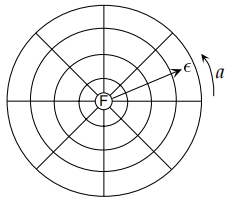
\includegraphics[scale=0.4]{./png/sphericalCoord}
  \end{center}
  The north pole is located at the fixation point, the latitude coordinate is called the \emph{eccentricity} $\epsilon$, and the longitude coordinate, measured from the horizontal meridian, is called the \emph{azimuth} $a$.
\end{defn}

\begin{prin}
  \label{prin:primaryVisualCortexRepresent}
  In primary visual cortex, the visual world is split in half, with the region $-90^{\circ} \leq a \leq 90^{\circ}$ for $\epsilon$ from $0^{\circ}$ to about $70^{\circ}$ (for both eyes) represented on the left side of the brain, and the reflection of this region about the vertical meridian represented on the right side of the brain.
\end{prin}

%\begin{defn}
 % \label{def:tangentScreen}
  %A flat screen that does not coincide exactly with the sphere defined in Definition \ref{def:sphericalCoord} is called a \emph{tangent screen}.
%\end{defn}

\begin{defn}
  \label{defn:PolarCoord}
  % Polar and Cartesian coordinate systems used to parameterize image location is shown in the following figure. Each rectangle represents a tangent screen, and the filled circle is the location of a particular image point on the screen.
  Polar coordinate system used to parameterize image location is shown in the following figure.
  \begin{center}
    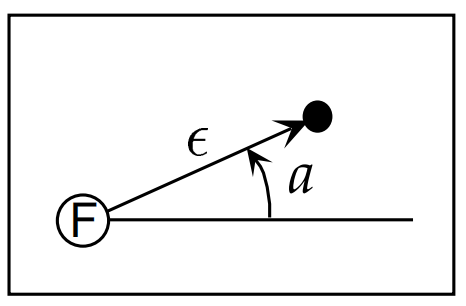
\includegraphics[scale=0.15]{./png/polarCoord}
  \end{center}
  The rectangle represents a \emph{tangent screen}, the filled circle is the location of a particular image point on the screen, the origin of the polar coordinate system is the fixation point $F$, the \emph{eccentricity} $\epsilon$ is proportional to the radial distance from the fixation point to the image point, and $a$ is the angle between the radial line from $F$ to the image point and the horizontal axis.
\end{defn}

\begin{rem}
  In most experiments, images are displayed on a tangent screen that does not coincide exactly with the sphere discussed in the previous paragraph. However, if the tangent screen is not too large, the difference is negligible, and the eccentricity and azimuth angles approximately coincide with polar coordinates on the screen.
\end{rem}

\begin{asm}
  \label{asm:unit}
  The eccentricity $\epsilon$ and the $x$ and $y$ coordinates of the Cartesian system that are based on measuring distances on the screen are converted to degrees by
  \begin{equation}
    \label{equ:conversion}
    \frac{l}{r}\times\frac{180^{\circ}}{\pi},
  \end{equation}
  where $l$ is the distance on the screen, $r$ is the distance from the eye to the screen.
\end{asm}

\begin{rem}
  Assumption \ref{asm:unit} makes sense because it is the angular, not the absolute size and location of an image that is typically relevant for studies of the visual system. And Equation \ref{equ:conversion} is similar to the arc length-radian relationship.
\end{rem}

\begin{exm}
  \label{exm:cortexImage}
  The following figure shows An autoradiograph of the posterior region of the primary visual cortex from the left side of a macaque monkey brain. The pattern is a radioactive trace of the activity evoked by an image like that in Definition \ref{def:sphericalCoord} figure. The vertical lines correspond to circles at eccentricities of $1^{\circ}$, $2.3^{\circ}$, and $5.4^{\circ}$, and the horizontal lines (from top to bottom) represent radial lines in the visual image at a values of $-90^{\circ}$, $-45^{\circ}$, $0^{\circ}$, $45^{\circ}$, and $90^{\circ}$. Only the part of cortex corresponding to the central region of the visual field on one side is shown.
  \begin{center}
    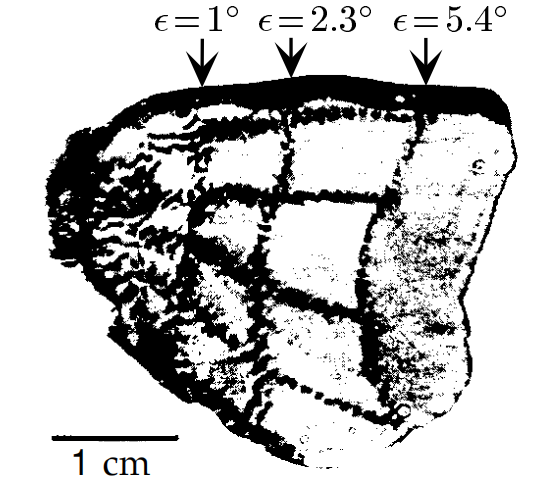
\includegraphics[scale=0.2]{./png/exm_cortexImage}
    %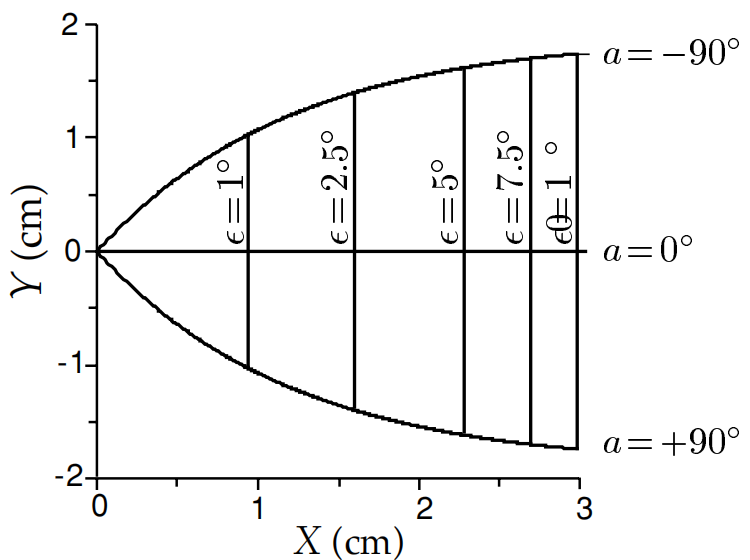
\includegraphics[scale=0.15]{./png/exm_retinotopicMap}
  \end{center}
\end{exm}

\begin{rem}
  \label{mapOnto}
  To construct the retinotopic map, we assume that eccentricity is mapped onto the horizontal coordinate $X$ of the cortical sheet, and $a$ is mapped onto its $Y$ coordinate.
\end{rem}

\begin{defn}
  \label{def:corticalMagnificationFactor}
  The \emph{cortical magnification factor} determines the distance across a flattened sheet of cortex separating the activity evoked by two nearby image points.
\end{defn}

\begin{asm}
  \label{asm:isotropic}
  We assume the cortical magnification factor is isotropic, denoted by $M(\epsilon)$.
\end{asm}

\begin{exm}
  Suppose that there are two image points in question $(\epsilon,a)$ and $(\epsilon+\Delta\epsilon,a)$, the angular distance between these two points is $\Delta\epsilon$, and the distance separating the activity evoked by these two image points on the cortex is $\Delta X$. By the definition of $M(\epsilon)$, these two quantities satisfy $\Delta X = M(\epsilon)\Delta\epsilon$ or, taking the limit as $\Delta X$ and $\Delta\epsilon$ go to $0$,
  \begin{equation}
    \label{equ:2.13}
    \frac{dX}{d\epsilon} = M(\epsilon).
  \end{equation}
  Suppose that there are the other two image points in question $(\epsilon,a)$ and $(\epsilon,a+\Delta a)$, the angular distance between these two points is
  \begin{displaymath}
    \Delta a \times\frac{\epsilon\pi}{180^{\circ}},
  \end{displaymath}
  where $\epsilon$ corrects for the increase of arc length as a function of eccentricity, and $\frac{\pi}{180^{\circ}}$converts from degrees to radians. The separation on the cortex $\Delta Y$ corresponding to these points satisfies $\Delta Y = \Delta a \frac{\epsilon\pi}{180^{\circ}}M(\epsilon)$. Taking the limit $\Delta a \to 0$,
  \begin{equation}
    \label{equ:2.16}
    \frac{dY}{da} = -\frac{\epsilon\pi}{180^{\circ}}M(\epsilon).
  \end{equation}
  The minus sign in this relationship appears because the visual field is inverted on the cortex.
\end{exm}

\begin{exm}
  \label{exm:macaqueMonkey}
  The cortical magnification factor for the macaque monkey, obtained from results such as the figure in Example \ref{exm:cortexImage}, is approximately
  \begin{equation}
    \label{equ:2.14}
    M(\epsilon) = \frac{\lambda}{\epsilon_0+\epsilon},
  \end{equation}
  with $\lambda \approx 12$ mm and $\epsilon_0 \approx 1^{\circ}$. Integrating Equation \ref{equ:2.13} and defining $X = 0$ to be the point representing $\epsilon = 0$, we find
  \begin{equation}
    \label{equ:2.15}
    X = \lambda \ln(1+\frac{\epsilon}{\epsilon_0}).
  \end{equation}
  Similarly,
  \begin{equation}
    \label{equ:2.17}
    Y = -\frac{\lambda\epsilon a \pi}{(\epsilon_0+\epsilon)180^{\circ}}.
  \end{equation}
  The following figure shows that these coordinates agree fairly well with the map in Example \ref{exm:cortexImage}.
  \begin{center}
    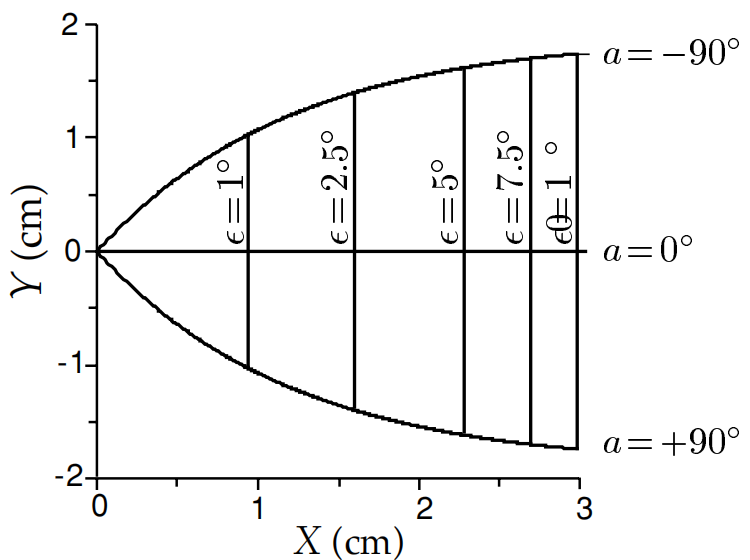
\includegraphics[scale=0.2]{./png/exm_retinotopicMap}
  \end{center}
\end{exm}

\begin{exm}
  For $\epsilon \gg 1^{\circ}$, equations \ref{equ:2.15} and \ref{equ:2.17} reduce to
  \begin{displaymath}
    X \approx \lambda\ln(\frac{\epsilon}{\epsilon_0}),
    Y \approx -\frac{\lambda \pi a}{180^{\circ}}.
  \end{displaymath}
  These two formulas can be combined by defining the complex numbers
  $Z = X+iY$ and $z = \frac{\epsilon}{\epsilon_0}\exp\left(-i\pi a/180^{\circ}\right)$, and writing
  \begin{displaymath}
    Z = \lambda\ln(z).
  \end{displaymath}
  For this reason, the cortical map is sometimes called a \emph{complex logarithmic map}.

  For an image scaled radially by a factor $\gamma$, eccentricities change according to $\epsilon \to \gamma \epsilon$ while $a$ is unaffected. Scaling of the eccentricity produces a shift
  \begin{displaymath}
    X \to X+\lambda\ln(\gamma)
  \end{displaymath}
  over the range of values where the simple logarithmic form of the map is valid. The logarithmic transformation thus causes images that are scaled radially outward on the retina to be represented at locations on the cortex translated in the $X$ direction.
\end{exm}

\begin{rem}
  For smaller $\epsilon$, the map we have derived is only approximate even in the complete form given by equations \ref{equ:2.15} and \ref{equ:2.17}. This is because the cortical magnification factor is not really isotropic, as we have assumed in this derivation, and a complete description requires accounting for the curvature of the cortical surface.
\end{rem}

\subsection{Visual Stimuli}
\label{sec:visualStimuli}
\begin{rem}
  Pixel locations are parameterized by Cartesian coordinates $x$ and $y$. However, pixel-by-pixel light intensities are not a useful way of parameterizing a visual image for the purposes of characterizing neuronal responses. This is because visually responsive neurons, like many sensory neurons, adapt to the overall level of screen illumination.
\end{rem}

\begin{defn}
  \label{defn:stimulusForm}
  we describe the \emph{visual stimulus} by a function $s(x,y,t)$ that is proportional to the difference between the luminance at the point $(x,y)$ at time $t$ and the average or background level of luminance.
\end{defn}

\begin{rem}
  Definition \ref{defn:stimulusForm} could avoid dealing with adaptation effects.
\end{rem}

\begin{defn}
  \label{def:contrast}
  The \emph{contrast} is the resulting quantity that $s(x,y,t)$ divided by the background luminance level, making it dimensionless.
\end{defn}
\begin{defn}
  \label{def:counterphaseSinusoidalGrating}
  A commonly used stimulus, the \emph{counterphase sinusoidal grating}, is described by
  \begin{equation}
    \label{equ:2.18}
    s(x,y,t) = A\cos(Kx\cos\Theta + Ky\sin\Theta-\Phi)\cos(\omega t),
  \end{equation}
  where $K$ and $\omega$ are the \emph{spatial} and \emph{temporal frequencies} of the grating (these are angular frequencies), $\Theta$ is its \emph{orientation}, $\Phi$ is its \emph{spatial phase}, and $A$ is its \emph{contrast amplitude}.
\end{defn}

\begin{exm}
  The following figure shows a similar grating (a spatial square wave is drawn rather than a sinusoid) and illustrates the significance of the parameters in Definition \ref{def:counterphaseSinusoidalGrating}. The lighter stripes are regions where $s>0$, and $s<0$ within the darker stripes.
  This stimulus oscillates in both space and time:
  \begin{enumerate}[(i)]
  \item At any fixed time, it oscillates in the direction perpendicular to the orientation angle $\Theta$ as a function of position, with wavelength $\frac{2\pi}{K}$ (figure A). A stimulus with $\Theta = 0$ varies in the x direction.
  \item At any fixed position, it oscillates in time with period $\frac{2\pi}{\omega}$ (figure B).
  \end{enumerate}
  Changing $\Phi$ by an amount $\Delta\Phi$ shifts the grating
  in the direction perpendicular to its orientation by a fraction $\frac{\Delta\Phi}{2\pi}$ of its wavelength, that is, $\frac{\Delta\Phi}{K}$, derived from
  \begin{displaymath}
    \begin{aligned}
      &\ \ \ \ Kx\cos\Theta + Ky\sin\Theta-(\Phi+\Delta\Phi)\\
      &= Kx\cos\Theta + Ky\sin\Theta - \Delta\Phi(\sin\Theta^2+\cos\Theta^2) -\Phi\\
      &= K(x-\frac{\Delta\Phi}{K}\cos\Theta)\cos\Theta + K(y-\frac{\Delta\Phi}{K}\sin\Theta)\sin\Theta-\Phi.
    \end{aligned}
  \end{displaymath}
  The contrast amplitude $A$ controls the maximum degree of difference between light and dark areas.
  \begin{center}
    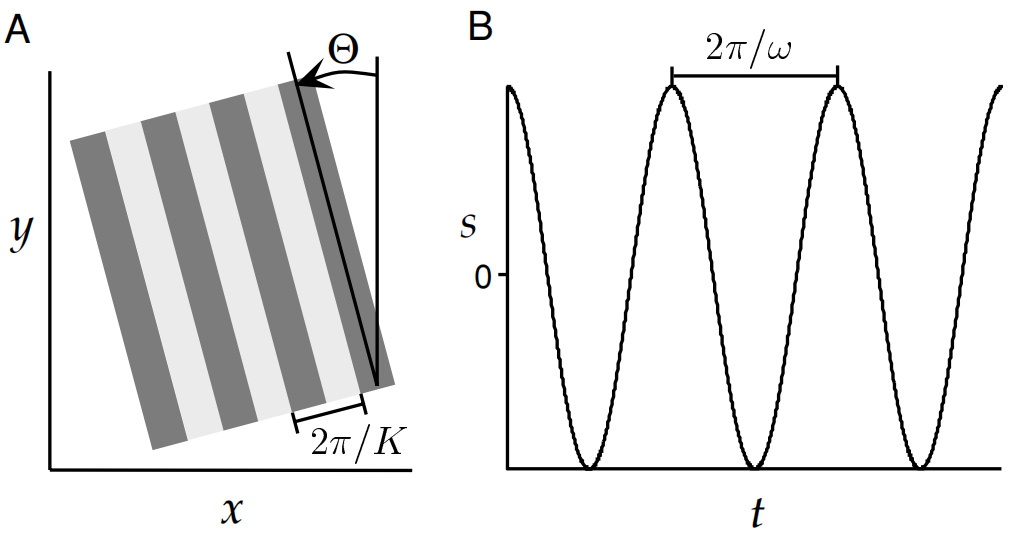
\includegraphics[scale=0.2]{./png/squareWave}
  \end{center}
\end{exm}

\begin{exc}
  Prove that units of parameters in Definition \ref{def:counterphaseSinusoidalGrating} are as follows:
  \begin{center}
    \renewcommand\arraystretch{1.8}
    \begin{tabular}[h]{|c|c|}
      \hline
      parameter & unit \\
      \hline
      $K$ & radians per degree\\
      \hline
      $\frac{K}{2\pi}$ & cycles per degree \\
      \hline
      $\Phi$ & radians \\
      \hline
      $\omega$ & radians/s(second) \\
      \hline
      $\frac{\omega}{2\pi}$ & HZ \\
      \hline
    \end{tabular}
  \end{center}
\end{exc}

\begin{rem}
  Experiments that consider reverse correlation and spike-triggered averages use various types of random and white-noise stimuli in addition to bars and gratings.
\end{rem}

\begin{defn}
  \label{def:whiteNoiseImage}
  A \emph{white-noise image} is one visual stimulus that is uncorrelated in both space and time so that
  \begin{equation}
    \label{equ:2.19}
    \frac{1}{T}\int_0^Ts(x,y,t)s(x',y',t+\tau)dt = \sigma_s^2\delta(\tau)\delta(x-x')\delta(y-y').
  \end{equation}
\end{defn}

\begin{rem}
  In practice a discrete approximation of such a stimulus must be used by dividing the image space into pixels and time into small bins. In addition, more structured random sets of images (randomly oriented bars, for example) are sometimes used to enhance the responses obtained during stimulation.
\end{rem}

\subsection{The Nyquist Frequency}
\label{sec:NyquistFrequency}
\begin{rem}
  Many factors limit the maximal spatial frequency that can be resolved by the visual system, one interesting effect arises from the size and spacing of individual photoreceptors on the retina.  The region of the retina with the highest resolution is the fovea at the center of the visual field. Within the macaque or human fovea, cone photoreceptors are densely packed in a regular array.
\end{rem}

\begin{defn}
  Along any direction in the visual field, a regular array of tightly packed photoreceptors of size $\Delta x$ samples points at locations $m\Delta x$ for $m = 1,2,\dots$. The (angular) frequency that defines the \emph{resolution} of such an array is called the \emph{Nyquist frequency} and is given by
  \begin{equation}
    \label{equ:2.20}
    K_{\rm{nyq}} = \frac{\pi}{\Delta x}.
  \end{equation}
\end{defn}

\begin{exm}
  \label{exm:nyqFrequency}
  Consider sampling two cosine gratings with spatial frequencies of $K$ and $2K_{\rm{nyq}}-K$, with $K < K_{\rm{nyq}}$. These are described by $s = \cos(Kx)$ and $s = \cos((2K_{\rm{nyq}}-K)x)$. At the sampled points $m\Delta x$, these functions are identical because
  \begin{displaymath}
    \cos((2K_{\rm{nyq}}-K)m\Delta x) = \cos(2\pi m - Km\Delta x) = \cos(Km\Delta x),
  \end{displaymath}
  which follows from the periodicity and evenness of the cosine function (see the following figure).
  \begin{center}
    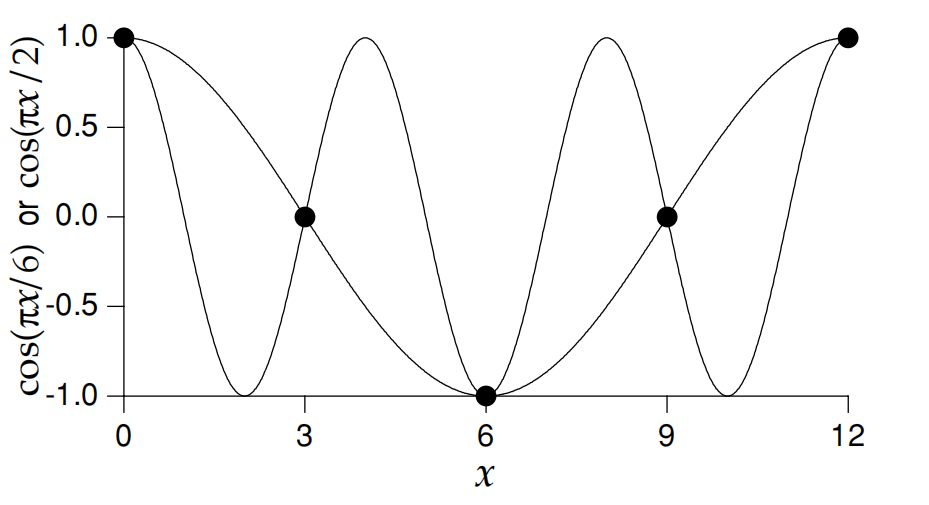
\includegraphics[scale=0.2]{./png/NyqFrequency}
  \end{center}
  As a result, these two gratings cannot be distinguished by examining them only at the sampled points.
  %The dots show points sampled with a spacing of $\Delta x = 3$. The Nyquist frequency in this case is $\pi/3$, and the two cosine curves match at the sampled points because their spatial frequencies satisfy the relation $2\pi/3-\pi/6 = \pi/2$.
\end{exm}

\begin{rem}[The importance of Nyquist frequency]
  As discussed in Example \ref{exm:nyqFrequency}, any two spatial frequencies $K < K_{\rm{nyq}}$ and $2K_{\rm{nyq}}-K$ can be confused with one another in this way, a phenomenon known as aliasing. Conversely, if an image is constructed solely of frequencies less than $K_{\rm{nyq}}$, it can be reconstructed perfectly from the finite set of samples provided by the array. (Note that, images with smaller $K$ will be easier to distinguish because of their bigger wavelengths.)
\end{rem}

\begin{exm}
  There are $120$ cones per degree at the fovea of the macaque retina, which makes $\Delta x = 1/120$ and
  \begin{displaymath}
    \frac{K_{\rm{nyq}}}{2\pi} = \frac{1}{2\Delta x} = 60 \ \rm{cycles\ per\ degree}.
  \end{displaymath}
  In this result, we have divided the right side of Equation \ref{equ:2.20}, which gives $K_{\rm{nyq}}$ in units of radians per degree, by $2\pi$ to convert the answer to cycles per degree.
\end{exm}





 



 
 




%%% Local Variables:
%%% mode: latex
%%% TeX-master: "../notesOnFluidMechanics"
%%% End:
